\documentclass[smallextended]{svjour3}

\usepackage{graphicx,amsmath,amssymb,amsfonts}
\usepackage[margin=1in]{geometry}
\usepackage{hyperref}
\usepackage{natbib}
\usepackage{color}

\renewcommand{\bottomfraction}{1.}
\renewcommand{\topfraction}{1.}
\renewcommand{\textfraction}{0}
\renewcommand{\floatpagefraction}{1.}

\graphicspath{{../correlation_analysis/figures/}}

% definition of \customlabel, which is used to label supplementary figures and tables
\makeatletter
\newcommand{\customlabel}[2]{%
\protected@write \@auxout {}{\string \newlabel {#1}{{#2}{\thepage}{}{}{}}}}
\makeatother


\journalname{Preprint}

\begin{document}

\title{Predicting evolutionary site variability from structure in viral proteins: buriedness, flexibility, and design}
\titlerunning{Predicting evolutionary site variability from structure}

\author{Amir Shahmoradi \and Dariya K. Sydykova \and \\ Stephanie J. Spielman \and Eleisha L. Jackson \and \\ Eric T. Dawson \and Austin G. Meyer \and Claus O. Wilke}

\institute{Amir Shahmoradi \at Department of Physics, The University of Texas at Austin, TX, 78712. \\
\and
Amir Shahmoradi \and Dariya K. Sydykova \and Stephanie J. Spielman \and Eleisha L. Jackson \and Eric T. Dawson \and Austin G. Meyer \and Claus O. Wilke \at Department of Integrative Biology, Center for Computational Biology and Bioinformatics, and Institute for Cellular and Molecular Biology, The University of Texas at Austin, TX, 78712. \email{wilke@austin.utexas.edu} }

\date{}

\maketitle

\begin{abstract}
Several recent works have shown that protein structure can predict site-specific evolutionary sequence variation. In particular, sites that are buried and/or have many contacts with other sites in a structure have been shown to evolve more slowly than surface sites with few contacts. Here, we present a comprehensive study of the extent to which numerous structural properties can predict sequence variation. The structural properties we consider include buriedness (relative solvent accessibility and contact number), measures of structural fluctuations (B factors, root-mean-square fluctuations, and variation in dihedral angles), and variability in designed structures. We obtained structural fluctuation measures both from molecular dynamics simulations performed on 9 non-homologous viral protein structures and from variation in homologous variants of those proteins, where available. We obtained measures of variability in designed structures from flexible-backbone design in the Rosetta software. We found that most of the structural properties correlate with site variation in the majority of structures, though the correlations are generally weak (correlation coefficients of 0.1 to 0.4). Moreover, we found that measures of buriedness tend to be better predictors of evolutionary variation than are measures of structural fluctuations. Finally, variability in designed structures was a weaker predictor of evolutionary variability than were both buriedness and fluctuation measures. We conclude that simple measures of buriedness are better predictors of evolutionary variation than are more complicated predictors obtained from dynamic simulations, ensembles of homologous structures, or computational protein design.
\end{abstract}


\section*{Introduction}

Patterns of sequence variation in protein-coding genes are shaped by biophysical structure and function of the expressed proteins
\citep{WilkeDrummond2010,MarshTeichmann2014}. As the most basic reflection of this relationship, buried residues in proteins tend to be more evolutionarily conserved than exposed residues
\citep{Overingtonetal1992,Goldmanetal1998,MirnyShakhnovich1999,Deanetal2002}. More specifically, when evolutionary variation is plotted as a function of Relative Solvent Accessibility (RSA, a measure of residue buriedness), the relationship falls, on average, onto a straight line with a positive slope \citep{FranzosaXia2009,Ramseyetal2011,FranzosaXia2012,Scherreretal2012}. Importantly, however, this relationship represents an average over many sites and many proteins. At the level of individual sites in individual proteins, RSA is often only weakly correlated with evolutionary variation \citep{MeyerWilke2013,Meyeretal2013,Yehetal2014}.

Measures of residue buriedness other than RSA, such as residue contact number (CN) have also been shown to correlate with sequence variability \citep{Liaoetal2005,FranzosaXia2009,Yehetal2014}, and some have argued that CN predicts evolutionary variation better than RSA \citep{Yehetal2014}. Because CN may be a proxy of residue and site-specific backbone flexibility \citep{Halle2002}, a positive trend between local structural variability and sequence variability may also exist \citep{Yehetal2014}. Indeed, several authors have suggested that such protein dynamics may play a role in sequence variability \citep{LiuBahar2012,NevinGereketal2013,MarshTeichmann2014}. However, a recent paper argued against \texbtf{the flexibility model (from SJS perspective, unclear what this refers to)}, on the grounds that it could introduce certain non-linearities that are not observed in the data \citep{Huangetal2014}.

While RSA and CN can be calculated in a straightforward manner from individual crystal structures, measures of structural flexibility, either at the side-chain or the backbone level, are more difficult to obtain. Two strong candidates for measuring structural flexibility are examining existing structural data or simulating protein dynamics. First, NMR ensembles and/or PDB structures may approximate \emph{in vivo} physiologically relevant structural fluctuations well. Indeed, the thermal motion of atoms in a crystal are recorded in B factors, which are available for every atom in every PDB structure. However, it is unclear how accurately B factors reflect structural fluctuations of a protein in solution. It is also possible to align homologous PDB protein structures and subsequently assess the extent of fluctuations. Other than using existing structural information, one could measure protein fluctuations using a simulation approach, either using coarse-grained modeling, e.g. via Elastic Network Models \citep{Sanejouand2013}, or using atom-level modeling, e.g. via molecular dynamics (MD) \citep{KarplusMcCammon2002}. Even so, it is not well understood which, if any, of these measures of structural fluctuations provide distinct insight into the evolutionary process, in particular site-specific variation evolutionary variation.

Here, we provide a comprehensive analysis of the extent to which numerous different structural quantities predict evolutionary sequence (amino-acid) variation. 

 We consider two measures of evolutionary sequence variation: site entropy, as calculated from homologous protein alignments, and evolutionary rate. For structural predictors, we include both measures of buriedness (RSA and CN) and measures of structural fluctuations. The fluctuation measures include B factors, several measures of backbone and side-chain variability obtained from MD simulations, and backbone variability obtained from alignments of homologous crystal structures. We also include site variability, as predicted from computational protein design with Rosetta. We consider site variability to be a structural property since it was derived in an explicit protein design context. On a set of nine viral proteins, we find that measures of buriedness generally perform better at predicting evolutionary site variation than do either measures of structural fluctuations or computational protein design. Among the measures of structural fluctuations, measures of side-chain variability perform better than do measures of backbone variability, possibly because the former are more tightly correlated with residue buriedness. Finally, site variability predicted from computational protein design performs worse than the best-performing measures of structural fluctuations.


\section*{Materials and Methods}

\subsection*{Sequence data, alignments, and evolutionary rates}

All viral sequences except influenza sequences were retrieved from \url{http://hfv.lanl.gov/components/sequence/HCV/search/searchi.html}.
The sequences were truncated to the desired genomic region but not in any other way restricted. Influenza sequences were downloaded from \url{http://www.fludb.org/brc/home.spg?decorator=influenza}. We only considered human influenza A, H1N1, excluding H1N1 sequences derived from the 2009 Swine Flu outbreak. We only used sequences from after 1998 but did not place any geographic restrictions.
%HIV-1 sequences were retrieved from \url{http://www.hiv.lanl.gov/components/sequence/HIV/search/search.html}.
%Sequences were truncated to the desired genomic region, but no other restrictions were imposed.

For all viral sequences, we removed any sequence that was not in reading frame, any sequence which was shorter than 80\% of the longest sequence for a given viral protein (so as to remove all partial sequences), and any sequence containing any ambiguous characters. Alignments were constructed using amino-acid sequences with MAFFT \citep{Katohetal2002,Katohetal2005}, specifying the \verb+--auto+ flag to select the optimal algorithm for the given data set, and then back-translated to a codon alignment using the original nucleotide sequence data.

To assess site-specific sequence variability in amino-acid alignments, we calculated the Shannon entropy ($H_i$) at each alignment column $i$:
\begin{equation}
        H_i = - \sum_jP_{ij}\ln P_{ij},
\end{equation}
where $P_{ij}$ is relative frequency of amino acid $j$ at position $i$ in the alignment.

For each alignment, we also calculated evolutionary rates, as described \citep{SpielmanWilke2013}. In brief, we generated a phylogeny for each codon alignment in RAxML \citep{RaxMLHPC} using the GTRGAMMA model. Using the codon alignment and phylogeny, we inferred evolutionary rates with a Random Effects Likelihood (REL) model, using the HyPhy software \citep{KosakovskyPondetal2005}. The REL model was a variant of the GY94 evolutionary model \citep{GoldmanYang1994} with five $\omega$ rate categories as free parameters.  We employed an Empirical Bayes approach \citep{Yang2000} to infer $\omega$ values for each position in the alignment. These $\omega$ values represent the evolutionary-rate ratio $dN/dS$ at each site.


\subsection*{Protein crystal structures}

A total of 9 viral protein structures were selected for analysis, as tabulated in Table \ref{tab:pdb_names}. Sites in the PDB structures were mapped to sites in the viral sequence alignments via a custom-built python script that creates a consensus map between a PDB sequence and all sequences in an alignment.

For each of the viral proteins, homologous structures were identified using the \texttt{blast.pdb} function of the R package Bio3D \citep{Grantetal2006}. BLAST hits were retained if they had $\geq35$\% sequence identity and $\geq90$\% alignment length. Among the retained hits, we subsequently identified sets of homologous structures with unique sequences and with mutual pairwise sequence divergences of $\geq2\%$, $\geq5\%$, and $\geq10\%$.

\subsection*{Measures of buriedness and of structural flexibility}

As measures of residue buriedness, we calculated Relative Solvent Accessibility (RSA), contact number (CN), and weighted contact number (WCN). To calculate RSA, we first calculated the Accessible Surface Area (ASA) for each residue in each protein, using the DSSP software \citep{KabschSander1983}. We then normalized ASA values by the theoretical maximum ASA of each residue \citep{Tienetal2013} to obtain RSA. We calculated CN for each residue as the total number of C$\alpha$ atoms surrounding the  C$\alpha$ atom of the focal residue within a spherical neighborhood of a predefined radius $r_0$. Following \citet{Yehetal2014}, we used $r_0=13\AA$. We calculated WCN as the total number of surrounding C$\alpha$ atoms for each focal residue, weighted by the inverse square separation between the C$\alpha$ atoms of the focal residue and the contacting residue, respectively \citep{Shihetal2012}.

In most analyses, we actually used the inverse of CN and/or WCN, $\text{iCN}=1/\text{CN}$ and $\text{iWCN}=1/\text{WCN}$. Note that for Spearman correlations, which we use throughout here, replacing a variable by its inverse changes the sign of the correlation coefficient but not the magnitude.

As measures of structural variability, we considered RMSF, variability in backbone and side-chain dihedral angles, and B factors. We calculated RMSF for backbone C$\alpha$ atoms based on both MD trajectories and homologous structures. For MD trajectories, we calculated RMSF as
\begin{equation}
    \text{RMSF}_j = \Big[\sum_i \big(\mathbf{r}_i^{(j)}-\mathbf{r}_0^{(j)}\big)^2\Big]^{1/2}
\end{equation}
where $\text{RMSF}_j$ is the root-mean-square fluctuation at site $j$, $\mathbf{r}_i^{(j)}$ is the position of the C$\alpha$ atom of residue $j$ at MD frame $i$, and $\mathbf{r}_0^{(j)}$ is the position of the C$\alpha$ atom of residue $j$ in the original crystal structure.

To calculate RMSF from homologous structures, we first aligned the structures using the Bio3D package \citep{Grantetal2006}, and then we calculated
\begin{equation}
    \text{RMSF}_j = \Big[\sum_i w_i\big(\mathbf{r}_i^{(j)}-\langle\mathbf{r}^{(j)}\rangle\big)^2\Big]^{1/2},
\end{equation}
where $\mathbf{r}_i^{(j)}$ now stands for the position of the C$\alpha$ atom of residue $j$ in structure $i$, $\langle\mathbf{r}^{(j)}\rangle$ is the mean position of that C$\alpha$ atom over all aligned structures, and $w_i$ is a weight to correct for potential phylogenetic relationship among the aligned structures. The weights $w_i$ were calculated using BranchManager \citep{StoneSidow2007}, based on phylogenies built with RAxML as before.

To assess variability in backbone and side-chain dihedral angles, we calculated Var($\phi$), Var($\psi$), and Var($\chi_1$). The variance of a dihedral angle was defined according to the most common definition in directional statistics:  
First, a unit vector $\mathbf{x}_i$ is assigned to each dihedral angle $\alpha_i$ in the sample. The unit vector is defined as $\mathbf{x}_i = ( \cos (\alpha_i), \sin (\alpha_i) )$.
The variance of the dihedral angle is then defined as
\begin{equation}
\text{Var}(\alpha) = 1 - ||\langle \mathbf{x}\rangle||,
\end{equation}
where $||\langle \mathbf{x}\rangle||$ represents the length of the mean $\langle \mathbf{x}\rangle$, calculated as $\langle \mathbf{x}\rangle=\sum_i \mathbf{x}_i/n$. Here, $n$ is the sample size. The variance of a dihedral angle is, by definition, a real number in the range $[0,1]$, with $\text{Var}(\alpha) = 0$ corresponding to the minimum variability of the dihedral angle and $\text{Var}(\alpha) = 1$ to the maximum, respectively \citep{Berens2009}. Since the $\chi_1$ angle is undefined for Ala and Gly we excluded all sites with these residues in analyses involving $\chi_1$.

B factors were extracted from the crystal structures. We only considered the B factors of the C$\alpha$ atom of each residue.


\subsection*{Molecular Dynamics Simulations}

Molecular dynamics (MD) simulations were carried out using the GPU implementation of the {\it Amber12} simulation package \citep{SalomonFerreretal2013} with the most recent release of the Amber fixed-charge force field (ff12SB; c.f., AmberTools13 Manual). Prior to MD production runs, all PDB structures were first solvated in a box of TIP3P water molecules \citep{jorgensen1983} such that the structures were  at least $10\AA$ away from the box walls. Each individual system was then energy minimized using the steepest descent method for 1000 steps, followed by conjugate gradient for another 1000 steps. Then, the structures were constantly heated from 0K to 300K for 0.1ns, followed by 0.1ns constant pressure simulations with positional harmonic restraints on all atoms to avoid instabilities during the equilibration process. The systems were then equilibrated for another 5ns without positional restraints, each followed by 15ns of production simulations for subsequent post-processing and analyses. All equilibration and production simulations were run using the SHAKE algorithm \citep{Ryckaert1977}. Langevin dynamics were used for temperature control.

\subsection*{Sequence Entropy from Designed Proteins}

Designed entropy was calculated as described \citep{Jacksonetal2013}. In brief, proteins were designed using RosettaDesign (Version 39284) \citep{LeaverFayetal2011} using a flexible backbone approach. This was done for all PDB structures in Table \ref{tab:pdb_names} as initial template structures. For each template, we created a backbone ensemble using the Backrub method \citep{Smith2008}. The temperature parameter in Backrub was set to 0.6, allowing for an intermediate amount of flexibility.  For each of the 9 template structures we designed 100 proteins.

\subsection*{Availability of data and methods}

All details of simulations, input$/$output files, and scripts for subsequent analyses are available to view or download at \url{https://github.com/clauswilke/structural\_prediction\_of\_ER}.

\section*{Results}

\subsection*{Data set and structural variables considered}

Our goal in this work is to determine which structural properties best predict amino-acid variability at individual sites in proteins. To this end, we selected 9 viral proteins for which we had both high-quality crystal structures and abundant sequences to assess evolutionary variability (Table~\ref{tab:pdb_names}). We quantified evolutionary variability in two ways, by calculating entropies for each alignment column (sequence entropy) and by calculating the evolutionary-rate ratio $\omega=dN/dS$ (see Methods for details). Throughout this paper, we primarily report results obtained for sequence entropy. Results for $\omega$ are largely comparable, with some specific caveats detailed below.

As predictors of evolutionary variability, we considered two broad classes of structural properties, residue buriedness and residue flexibility, and we also considered the variability seen in computationally designed protein variants. Measures of buriedness quantify the extent to which a residue is protected from solvent. A commonly used measure of buriedness is solvent-accessible surface area (ASA) or its normalized variant relative solvent accessibility (RSA). Here we considered RSA, since it can be compared among residues of different sizes. We also considered contact number (CN) and weighted contact number (WCN). Both of these quantities assess the number of other residues a focal residue contacts. CN simply counts the number of contacts within a sphere of a given radius around the $\alpha$-carbon of the focal residue. WCN weights contacts by the distance between the two residues. Note that residue buriedness decreases as RSA increases, but it increases with increasing CN or WCN. To avoid this difference in directionality, in most analyses we replaced CN and WCN with their inverse, $\text{iCN}=1/\text{CN}$ and $\text{iWCN}=1/\text{WCN}$. Because nearly all analyses we carried out were non-parametric and only depended on the rank order of the variables, this substitution only changed the sign of correlations but not the magnitude.

Measures of flexibility assess the extent to which a residue fluctuates in space as a protein undergoes thermodynamic fluctuations in solution. There are different ways to quantify these fluctuations. First, we can measure the root mean-square deviation of the C$\alpha$ atom over time. This quantity is commonly called RMSF. Second, we can consider B factors, which measure the spatial localization of individual atoms in a protein crystal. Third, we can measure the variability in side-chain or backbone dihedral angles, such as Var($\chi_1$), Var($\phi$), or Var($\psi$). Here, we considered all these measures of structural variability.

To calculate measures of flexibility, we generated molecular-dynamics (MD) trajectories for all crystal structures in Table~\ref{tab:pdb_names}. In all cases, we equilibrated the structure and then simulated 15ns of chemical time (see Methods). We recorded snapshots of the simulated structure every 10ps. From these snapshots, for each residue we calculated RMSF as well as the variability in dihedral and side-chain angles. We also calculated time-averaged values of the three measures of buriedness RSA, CN, and WCN. We refer to these time-averaged values as MD RSA, MD CN, and MD WCN, respectively.

To assess variability in designed proteins, we used the Rosetta protein-design platform to generate 100 designed variants of each protein structure listed in Table~\ref{tab:pdb_names}. We then calculated the sequence entropy at each position in alignments of the designed variants. We refer to the resulting quantity as the \emph{designed entropy}. We had previously shown that designed entropy captures some but not all of the variation observed in natural alignments \citep{Jacksonetal2013}.

\subsection*{Structural buriedness vs.\ structural flexibility as predictors of evolutionary variation}

We first compared a subset of variables among the measures of buriedness and measures of fluctuations in their explanatory power for sequence variation. Figure~\ref{fig:cor_entropy_all} shows the Spearman correlation between sequence entropy and each of the quantities RSA, iWCN, Var$(\chi_1)$, RMSF, and B factor, for each protein. Significant correlations ($P<0.05$) are shown with filled symbols, and non-significant correlations are shown with empty symbols ($P\geq0.05$).
In this figure, several patterns emerge. First, all correlations are generally positive and significant. The main exception is the RNA binding domain of Marburg virus, PDB ID 4GHA, which mostly shows no correlation but shows a negative correlation between sequence entropy and the variability in the $\chi_1$ angle. Second, correlations are generally weak. No correlation coefficient exceeds 0.4. Third, on average the correlation strength decreases as we move from left to right in the figure. The two measures of buriedness, RSA and iWCN, show the strongest correlations. Their correlations are on average $\rho=0.23$ and $\rho=0.22$, respectively. The three fluctuation measures Var($\chi_1$), RMSF, and B factor exhibit weaker correlations, on average $\rho=0.14$, $\rho=0.11$, and $\rho=0.12$, respectively.

We next analyzed structural fluctuations more carefully, by comparing the correlations of entropy with six different measures of local structural flexibility.  We considered variations in the backbone and side-chain dihedral angles ($\phi$, $\psi$, and $\chi_1$), B factors, RMSF obtained from MD simulations, and RMSF obtained from crystal structures. For the latter quantity, we aligned homologous structures with distinct sequences, obtained from the PDB (see Methods and Table~\ref{tab:homologs} for details). The correlation strengths of these quantities with entropy are shown in Figure~\ref{fig:cor_entropy_SF}. We found that the variation in backbone dihedral angles, Var($\phi$) and Var($\psi$), explained the least variation in sequence entropy, while the variation in the side-chain dihedral angle Var($\chi_1$) explained, on average, more variation in sequence entropy than any other measure of structural flexibility. B factors and the two measures of RMSF explained on average approximately the same amount of variation in entropy, even though the results for individual proteins were somewhat discordant (see also next sub-section).

\subsection*{MD time-averages vs.\ crystal-structure snapshots}

For most analyses discussed so far, except analyses involving B factors or crystal RMSF, we averaged structural quantities over MD trajectories comprising 15ns of chemical time. This is not conventional practice for quantities such as RSA or contact numbers. Instead, most authors simply obtain these quantities from individual crystal structures. We therefore asked whether MD averages differed in any meaningful way from estimates obtained from crystal structures, and whether estimates from MD and from crystal structures different in their predictive power for sequence variability.

We found that RSA, CN, and WCN from crystal structures were highly correlated with their averages over MD trajectories, for all protein structures we examined (Spearman correlation coefficients of $>0.9$ in all cases, Table~\ref{tab:MDcrystal_cor}). Further, when we correlated these quantities with sequence entropy, we found that the correlation coefficients we obtained for each protein were virtually identical (Figure~\ref{fig:cor_cr_md}A-C). Thus, in terms of predicting evolutionary variation, RSA and contact numbers obtained from the static structures performed as well as their dynamic equivalents averaged over short time scales.

By contrast, we found more variation when we considered backbone flexibility as measured by root mean fluctuations (RMSF). RMSF cannot be obtained from a single crystal structure, but we can calculate it from an alignment of multiple crystal structures were available. When we compared RMSF from MD to RMSF from crystal structures, we found that they were sometimes quite different, with correlation coefficients ranging from 0.218 to 0.723 (Table~\ref{tab:MDcrystal_cor}). Consequently, for the two proteins for which MD RMSF was the least correlated with crystal-structure RMSF (hepatitis C protease and Rift Valley fever nucleoprotein), the strength of the correlation between site entropy and RMSF depended substantially on whether RMSF was obtained from MD or from crystal structures (Figures~\ref{fig:cor_entropy_SF} and~\ref{fig:cor_cr_md}D).

To further investigate the relationship between backbone fluctuations and sequence variability, we also compared the RMSF correlations to the correlations between sequence entropy and B factors. Again, we found that these correlations were generally different from the ones found for either the MD RMSF or the crystal structure RMSF (Figure \ref{fig:cor_entropy_bfca_rmsf}). Thus, B factors, MD RMSF, and crystal RMSF, though all measures of backbone fluctuations, contained distinct information about sequence variability in our data set.

\subsection*{Sequence entropy vs.\ evolutionary-rate ratio $\omega$}

In the previous subsections, we have used sequence entropy as a measure of amino-acid variability at individual sites. While sequence entropy is a simple and straightforward measure of site variability, it has two potential drawbacks: First, entropy doesn't correct for the phylogenetic relationship of sequences in the alignment, and hence it can be biased if some parts of the phylogeny are more densely sampled than others. Second, entropy does not take into account the actual substitution process. As a result, a single substitution near the root of the tree can result in a comparable entropy to a sequence of substitutions toggling back and forth between two amino acids.

To consider an alternative quantity of sequence variability that doesn't suffer from either of these drawbacks, we calculated the evolutionary-rate ratio $\omega=dN/dS$ for all proteins at all sites, and repeated all analyses with $\omega$ instead of entropy. We found that all results generally carried over, but the correlations tended to be somewhat weaker. Figure~\ref{fig:cor_entropy_omega} plots, for each protein, the correlation between $\omega$ and the various structural quantities versus the correlation between entropy and the same structural quantities. We see that all data points generally fall below the $x=y$ line, and are shifted downwards by approximately 0.1. Thus, correlations of structural quantities with $\omega$ are, on average, approximately 0.1 smaller than correlations of the same quantities with entropy.

Besides the measures of buriedness and measures of structural flexibility, we included in  Figure~\ref{fig:cor_entropy_omega} also the designed entropy.  We found that designed entropy performed about as well as the measures of structural flexibility did on average, but worse than the measures of buriedness, in predicting either $\omega$ or sequence entropy. Designed entropy will be discussed in more detail in the next subsection.

\subsection*{Multi-variate analysis of structural predictors}

The various structural quantities we have considered are by no means independent of each other. Measures of buriedness co-vary with each other, as do measures of structural flexibility. Further, the latter co-vary with the former, as does designed entropy. To determine the extent to which the various quantities contain independent information about sequence variability, and to assess whether combining multiple structural quantities yields improved predictive power, we carried out a joint multivariate analysis including most of the structural quantities considered in this work. The approach we used is a principal component (PC) regression, which has previously been used successfully to disentangle genomic predictors of whole-protein evolutionary rates \citep{Drummondetal2006,Bloometal2006}. In this analysis, we first carry out a principal component analysis of the predictor variables (i.e., the structural quantities such as RSA and RMSF), and we then regress the response (sequence entropy or $\omega$) against the individual components.

Because we wanted to analyze all proteins in our data set individually but in such a way that results were comparable from one protein to the next, we pooled all structural quantities for a single PC analysis and then regressed entropy and $\omega$ against each PC separately for each protein. The results of this analysis are shown in Figure~\ref{fig:cor_entropy_PC_screen}. The first component (PC1) explained on average the largest amount of variation in sequence entropy (see Figure~\ref{fig:cor_entropy_PC_screen}A). We found the second-highest $r^2$ values, on average, for PC3, while all other components explained very little variation in sequence entropy. When looking at the composition of the components, we found that RSA, iWCN, RMSF, and Var($\chi_1$) all loaded strongly on PC1, while PC2 and PC3 where primarily represented by designed entropy and B factors (see Figure~\ref{fig:cor_entropy_PC_screen}B and C). RMSF also had moderate loadings on PC3. Interestingly, designed entropy and B factors load with equal signs on PC2 but with opposite signs on PC3.

We think that PC1 can be considered as a buriedness component. By definition, PC1 measures the largest amount of variation among the structural quantities, and all structural quantities reflect to some extent the buriedness of residues. PC2 and PC3 are more difficult to interpret. Since designed entropy and B factors load strongly on both but with two different combinations of signs, we think the most parsimonious interpretation is to consider PC2 as a component representing sites with high designed entropy and high spatial fluctuations (as measured by B factors) and PC3 representing sites with high designed entropy and low spatial fluctuations. Using these interpretations, our PC regression analysis suggests that of all the structural quantities, residue buriedness is the best predictor of evolutionary variation. Designed entropy is a useful predictor as well, but it tends to perform better at sites with low spatial fluctuations.

When we included RMSF derived from crystal structures in our analysis, we found comparable results. The main differences occured in PC2 and PC3, where CS RMSF generally loaded in the opposite direction of B factor, and either in the same (PC2) or the opposite (PC3) direction of designed entropy (Figure~\ref{fig:cor_entropy_PC_screen_CSrmsf}). Finally, results were generally comparable when we considered $\omega$ instead of sequence entropy (Figures~\ref{fig:cor_omega_PC_screen} and~\ref{fig:cor_omega_PC_screen_CSrmsf}).

\section*{Discussion}

We have carried out a comprehensive analysis of how well structural quantities predict evolutionary variation in nine viral proteins. We have found that measures of buriedness generally performed better than measures of structural flexibility. Further, measures of buriedness also performed better than a computational protein-design approach that employed a sophisticated all-atom force field to determine allowed amino-acid distributions at each site. Finally, averaging structural quantities over 15ns of MD simulations provided no improvement in predictive power relative to taking the same quantities from individual crystal structures. 

Our results are broadly in agreement with recent work by Echave and collaborators \citep{Yehetal2014,Huangetal2014}. These authors found that RSA and contact number showed comparable correlation strengths with evolutionary variation \citep{Yehetal2014}. Further, they demonstrated that the observed relationship between evolutionary variation and residue--residue contacts was not consistent with a flexibility model that puts evolutionary variability in proportion to structural flexibility \citep{Huangetal2014}. Instead, a mechanistic stress model, in which amino-acid substitutions cause physical stress in proportion to the number of residue--residue contacts affected, could explain all the observed data \citep{Huangetal2014}.

We have found here that correlations between sequence entropy and structural quantities were consistently higher than correlations between the evolutionary-rate ratio $\omega$ and structural quantities. This difference likely reflects the distinct physical processes that entropy and $\omega$ measure. Entropy is a measure of the amino-acid diversity allowed at a given site. In effect, it reflects how many different amino acids are allowed. By contrast, $\omega$ measures how rapidly amino-acid changes occur at a given site. While entropy and $\omega$ are generally correlated, a site can have high entropy and comparatively low $\omega$ and vice versa. In particular, if mutations rapidly toggle back and forth between two different amino acids at a site, then that site will have high $\omega$ and low entropy. By contrast, if a site diversified into a number of different alleles deep in the phylogeny but did not experience much further evolution at later times, then that site will have comparatively high entropy but low $\omega$. Since structural quantities such as measures of buriedness reflect the biophysical constraints imposed on sites, it makes sense that they would be better predictors of the allowed amino-acid diversity at a site than the speed of substitution at that site. By contrast, biological processes such as immune escape would likely be better predictors of substitution rates than amino-acid diversity.

The correlation strengths we observed were consistently lower than those observed in prior work \citep{Jacksonetal2013,Yehetal2014}. We believe that this result was due to our choice of analyzing viral proteins instead of the cellular proteins or enzymes used in prior works. First, while viral sequences are abundant, their alignments may not be as diverged as alignments that can be obtained for sequences from cellular organisms. For example, our influenza sequences spanned only approximately one decade. Despite the high mutation rates observed in RNA viruses, the evolutionary variation that can accumulate over this time span is limited. And the lower the evolutionary divergence, the harder it becomes to resolve differences between more and less conserved sites. Second, many viral proteins experience a substantial amount of selection pressure to evade host immune responses. The resulting positive selection on viral sequences may mask evolutionary constraints imposed by structure. For example, influenza hemagglutinin displays positive selection throughout the entire sequence, and both at buried and at exposed sites \citep{MeyerWilke2013,Meyeretal2013,Suzuki2006,Bushetal1999}.

We found that simple measures of buriedness, such as RSA and contact numbers, were better predictors of evolutionary variation than sequence variability predicted from computational protein design. Thus, simple quantities that can be obtained trivially from PDB structures performed better than a sophisticated protein-design strategy that makes use of an all-atom energy function and requires thousands of CPU-hours to complete. This result highlights that even though computational protein design has yielded impressive results in specific cases \citep{Kuhlman2003,Rothlisberger2008,Fleishman2011}, it remains limited in its ability to predict evolutionary variation. We had previously found that flexible backbone design with Rosetta resulted in designs whose surface and core were too similar \citep{Jacksonetal2013}, and we had suggested that this discrepancy was caused either by the solvation model or the model of backbone flexibility we used (Backrub, see \citealt{Smith2008}). The results we found here suggest that the model of backbone flexibility may be the cause of at least some of the discrepancies between predicted and observed site variability. In particular, in our PC regression analysis we found that the component in which designed entropy loaded opposite to B factor and MD RMSF generally had the second-highest predictive power for evolutionary variability, after the component representing buriedness. Thus, designed entropy tended to perform better for sites with less structural variability.

Even though RSA and contact number remain the best currently known predictors of evolutionary variation, neither quantity has particularly high predictive power. One reason why predictive power may be low is that neither quantity accounts for correlated substitutions at interacting sites.  Yet such correlated substitutions happen regularly. For example, covariation among sites encodes information about residue-residue contacts and 3D structure \citep{Halabietal2009,BurgervanNimwegen2010,Marksetal2011,Jonesetal2014}, and evolutionary models that incorporate residue--residue interactions tend to perform better than models that do not \citep{Rodrigueetal2005,BordnerMittelmann2014}. An improved predictor of evolutionary variation would have to correctly predict this covariation from structure. In principle, computational protein design, which takes into consideration the atom-level details of the protein structure, should properly reproduce covariation among sites. However, a recent analysis showed that there are significant limitations to the covariation that is predicted \citep{OllikainenKortemme2013}. In addition, covariation in designed proteins is quite sensitive to the type of backbone variation modeled during design, and improved models of backbone flexibility may be required for improved prediction of covariation among sites \citep{OllikainenKortemme2013}.

\section*{Acknowledgments}

This work was supported in part by NIH grant R01 GM088344, DTRA grant HDTRA1-12-C-0007, ARO grant W911NF-12-1-0390, and the BEACON Center for the Study of Evolution in Action (NSF Cooperative Agreement DBI-0939454). The Texas Advanced Computing Center at UT Austin provided high-performance computing resources.

\bibliographystyle{spbasic}  % natbib.sty
\bibliography{Structural_prediction_of_ER}%%%refs.bib

\newpage

\section*{Tables}

\begin{table}[htbp]
\caption{PDB structures considered in this study.\label{tab:pdb_names}}
\smallskip

\centerline{
\begin{tabular}{c c c c c} % c}
                        \hline
    Viral Protein   &  PDB ID  & Chain    & Sequence  & Number of   \\ 
    &    &       & Length    & Sequences   \\\hline                                                           
  Hemagglutinin Precursor         & 1RD8           & AB        & 503                & 1039        \\
  Dengue Protease Helicase        & 2JLY           & A         & 451                & 2362        \\
  West Nile Protease              & 2FP7           & B         & 147                & 237         \\
  Japanese Encephalitis Helicase  & 2Z83           & A         & 426                & 145         \\
  Hepatitis C Protease            & 3GOL           & A         & 557                & 1021        \\
  %Hepatitis C Protease            & 3GSZ           & A         & 558                & 1021        \\
  %Hepatitis C Protease            & 3I5K           & A         & 566                & 1021        \\
  Rift Valley Fever Nucleoprotein & 3LYF           & A         & 244                & 95          \\
  Crimean Congo Nucleocapsid      & 4AQF           & B         & 474                & 69          \\
  Marburg RNA Binding Domain      & 4GHA           & A         & 122                & 42          \\
  Influenza Nucleoprotein         & 4IRY           & A         & 404                & 943         \\
  \hline
\end{tabular}
}
\end{table}

\begin{table}[htbp]
\caption{Availability of homologous crystal structures. Even though most viral proteins have many PDB structures available, the sequence divergence among these structures is low. To calculate RMSF from crystal structures, we here considered all proteins for which we could find at least five homologous structures at 5\% pairwise sequence divergence (highlighted in bold). \label{tab:homologs}}
\smallskip

\centerline{
\begin{tabular}{c c c c c c}
                        \hline
  Viral Protein & BLAST hits$^\text{a}$ & \multicolumn{4}{c}{Unique sequences} \\ 
    \cline{3-6}\noalign{\smallskip}
                &            & all  & $\geq2$\%$^\text{b}$  &  $\geq5$\%$^\text{b}$  & $\geq10$\%$^\text{b}$ \\\hline
  Hemagglutinin Precursor         & 63 & 17 & 10 & \textbf{9} & 7\\
  Dengue Protease Helicase        & 31 & 13 & 7 & \textbf{7} & 7\\
  West Nile Protease              & 21 & 16 & 10 & \textbf{7} & 6\\
  Japanese Encephalitis Helicase  & 31 & 12 & 7 & \textbf{7} & 7\\
  Hepatitis C Protease            & 302 & 33 & 10 & \textbf{5} & 4 \\
  Rift Valley Fever Nucleoprotein & 95  & 9 & 5 & \textbf{5} & 5\\
  Crimean Congo Nucleocapsid      & 7 & 4 & 3 & 2 & 2\\
  Marburg RNA Binding Domain      & 63 & 9 & 5 & 3 & 3\\
  Influenza Nucleoprotein         & 69 & 15 & 4 & 4 & 2\\
  \hline
\end{tabular}
}
$^\text{a}$ BLAST hits against all sequences in the PDB, excluding hits with $<35$\% sequence identity and $<90$\% alignment length\\
$^\text{b}$ Unique sequences at indicated minimum pairwise sequence divergence
\end{table}

\begin{table}[htbp]
\caption{Correlations between quantities obtained from MD trajectories and from crystal structures. For each quantity and each protein, we calculated the Spearman correlation $\rho$ between the values obtained from MD time averages and the values obtained from crystal structures. We then calculated the minimum, maximum, mean, and standard deviation of these correlations.\label{tab:MDcrystal_cor}}
\bigskip

\centerline{
\begin{tabular}{ccccc}
                        \hline
  Quantity    & min $\rho$ & max $\rho$ & $\langle\rho\rangle$ & SD($\rho$) \\\hline
  RSA       & 0.937 & 0.981 & 0.948 & 0.012\\
  CN        & 0.964 & 0.993 & 0.976 & 0.008\\
  WCN       & 0.973 & 0.991 & 0.984 & 0.006\\
  RMSF      & 0.218 & 0.723 & 0.502 & 0.181\\
  \hline
\end{tabular}
}

\end{table}

\clearpage

\section*{Figures}


\begin{figure}[tbh]
\begin{center}
    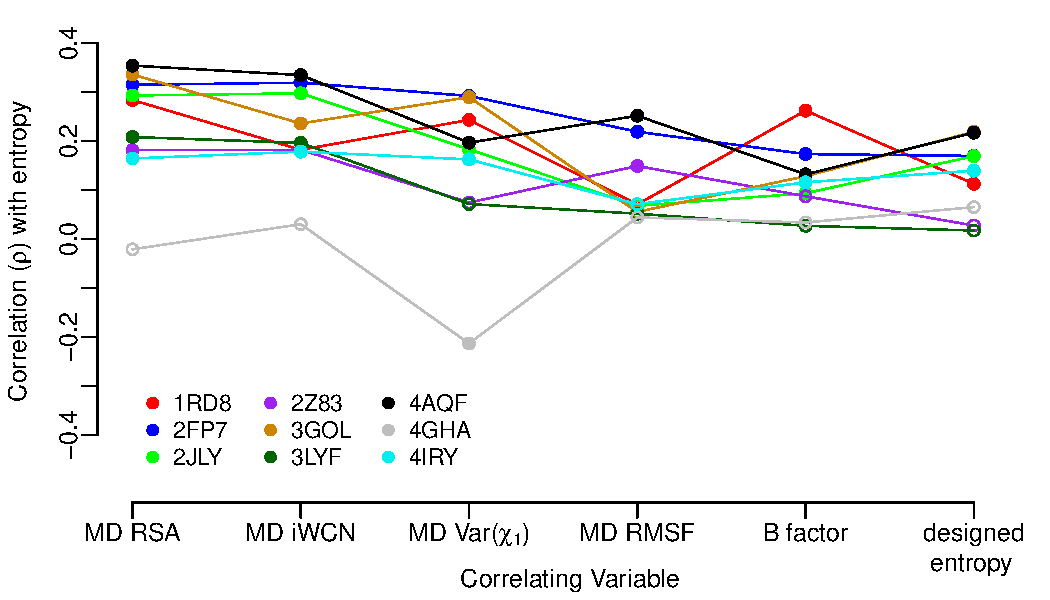
\includegraphics[width=5in]{cor_entropy_all.pdf}
\end{center}
\caption{Spearman correlation of sequence entropy with measures of buriedness and of structural variability. Each symbol represents one correlation coefficient for one protein structure. Significant correlations ($P<0.05$) are shown as filled symbols, and insignificant correlations ($P\leq0.05$) are shown as open symbols. The quantities RSA, iWCN, Var($\chi_1$), and RMSF were obtained as time-averages over 15ns of MD simulations. B factors were obtained from crystal structures. Compared to the measures of structural variability, the buriedness measures consistently show stronger correlations with sequence entropy.}
\label{fig:cor_entropy_all}
\end{figure}


\begin{figure}[tbh]
\begin{center}
    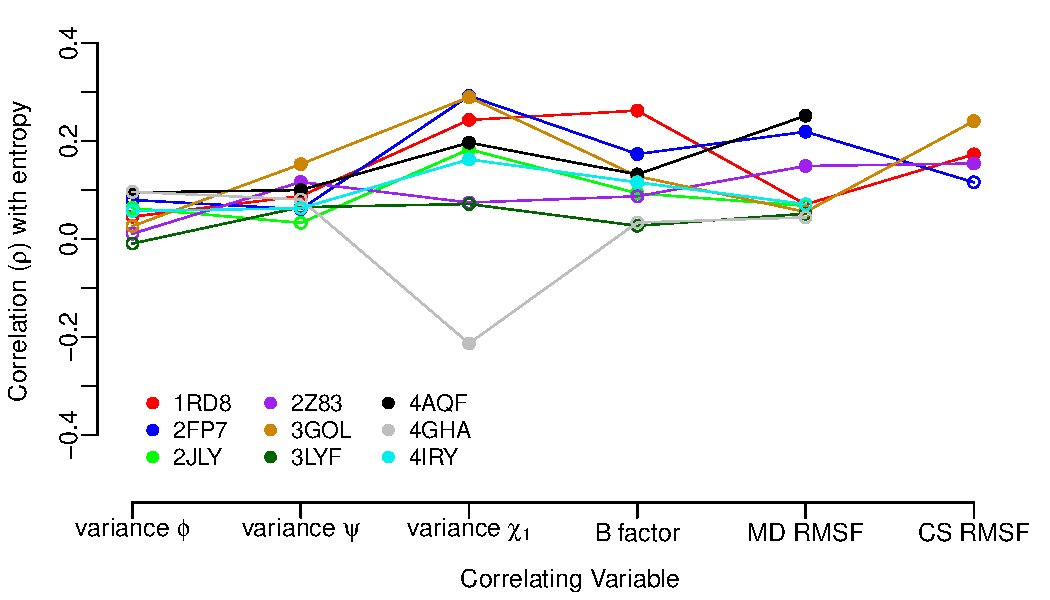
\includegraphics[width=5in]{cor_entropy_SF.pdf}
\end{center}
\caption{Spearman correlation of sequence entropy with measures of structural variability. Each symbol represents one correlation coefficient for one protein structure. Significant correlations ($P<0.05$) are shown as filled symbols, and insignificant correlations ($P\leq0.05$) are shown as open symbols. The quantities Var($\psi$), Var($\phi$), Var($\chi_1$), and MD RMSF were obtained as time-averages over 15ns of MD simulations. B factors were obtained from crystal structures. CS RMSF values were obtained from alignments of homologous crystal structures. Almost all structural measures of variability correlate weakly but significantly with sequence entropy.}
\label{fig:cor_entropy_SF}
\end{figure}

\begin{figure}[tbh]
\begin{center}
    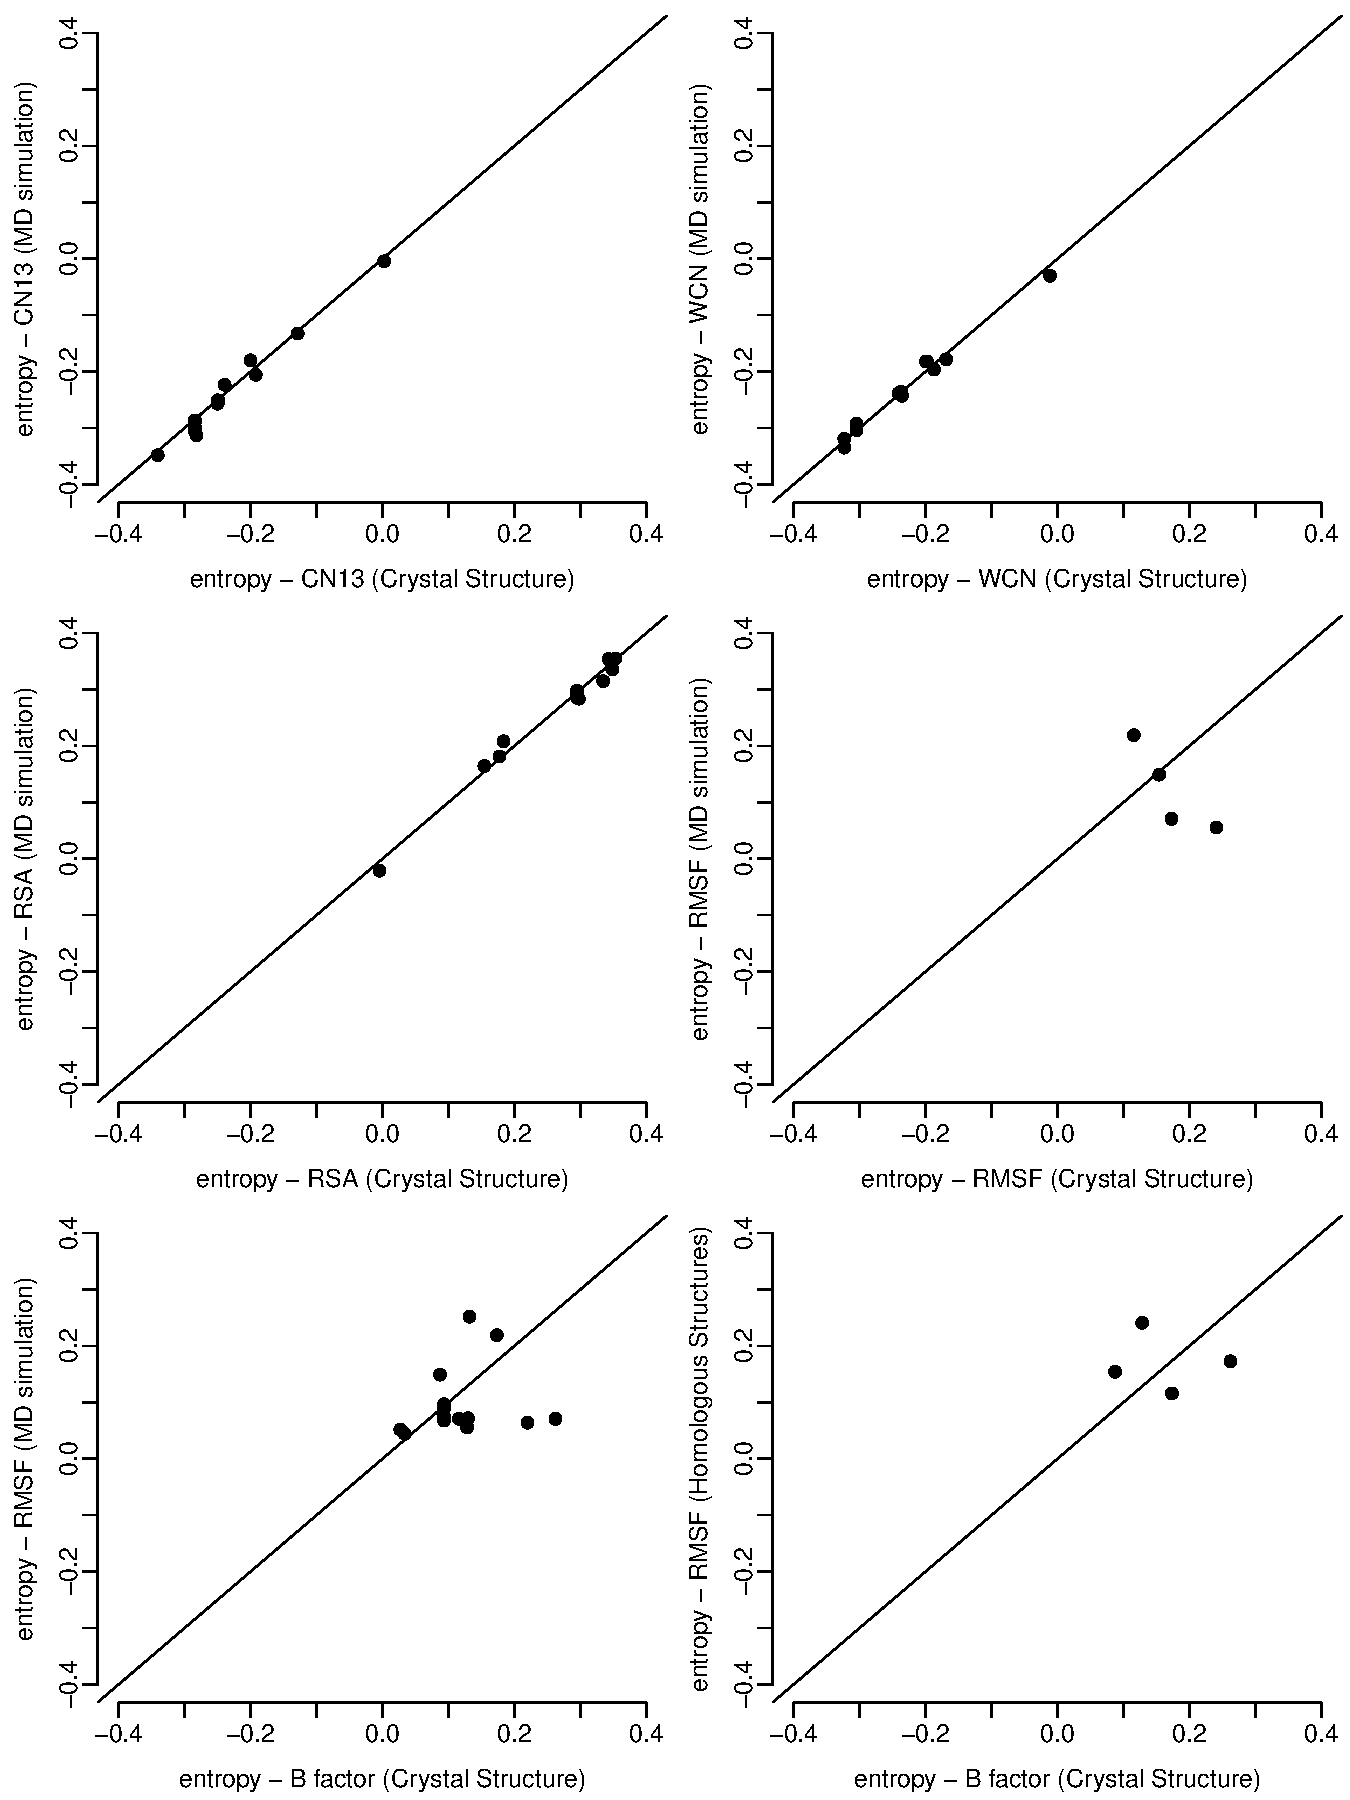
\includegraphics[width=6.5in]{cor_cr_md.pdf}
\end{center}
\caption{Spearman correlations of sequence entropy with MD-derived and crystal-structure derived structural measures.
The vertical axes in all plots represent the Spearman correlation of sequence entropy with one structural variable obtained from $15ns$ of Molecular Dynamics (MD) simulations. The horizontal axes represent the Spearman's rank correlation coefficient of sequence entropy with the same structural variable as in the vertical axes but measured from protein crystal structures. Each dot represents one correlation coefficient for one protein structure. The quantities iCN, iWCN, and RSA have nearly identical predictive power for sequence entropy regardless of whether they are derived from MD simulations or from crystal structures. By contrast, RMSF from MD simulations leads to very different correlations than RMSF from crystal structures does.
}
\label{fig:cor_cr_md}
\end{figure}

\begin{figure}[tbh]
\begin{center}
    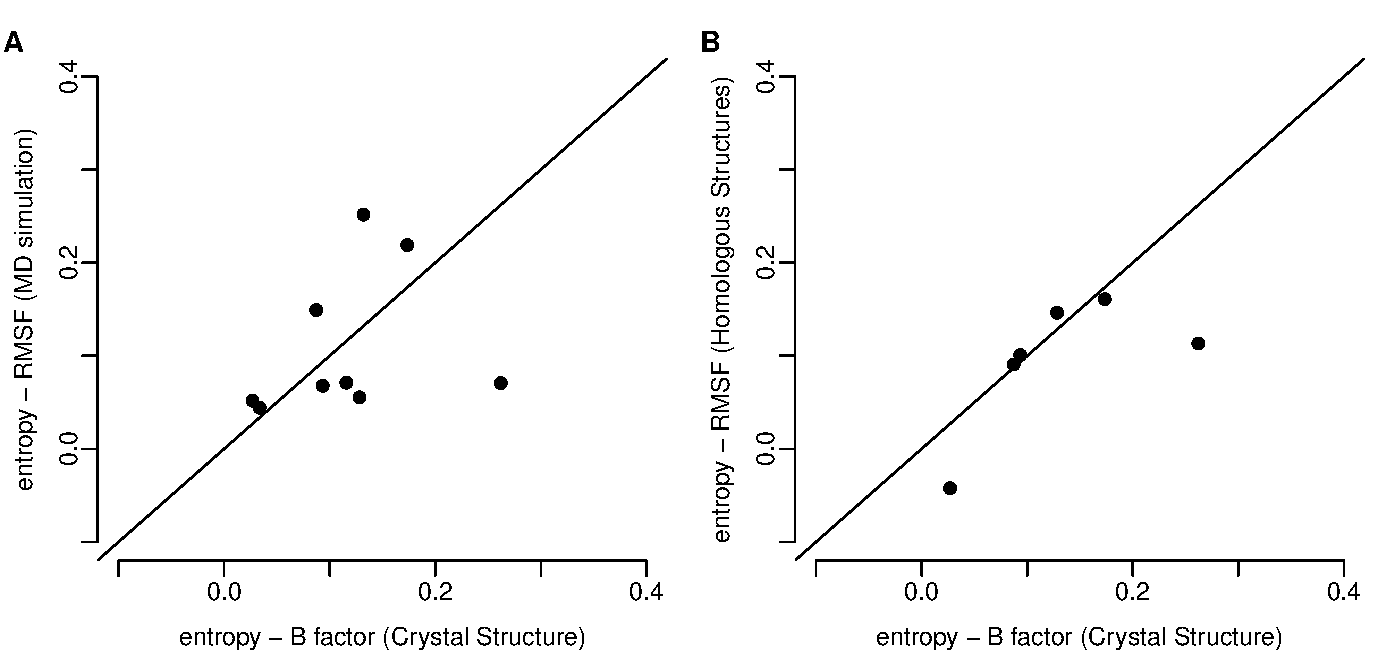
\includegraphics[width=6.5in]{cor_entropy_bfca_rmsf.pdf}
\end{center}
\caption{Spearman correlations of sequence entropy with measures of structural variability.
Vertical and horizonal axes represent Spearman correlations of the indicated quantities. Each dot represents one correlation coefficient for one protein structure. MD RMSF, crystal-structure RMSF, and B factors all explain different amounts of variance in sequence entropy for different proteins.}
\label{fig:cor_entropy_bfca_rmsf}
\end{figure}

\begin{figure}[tbh]
\begin{center}
    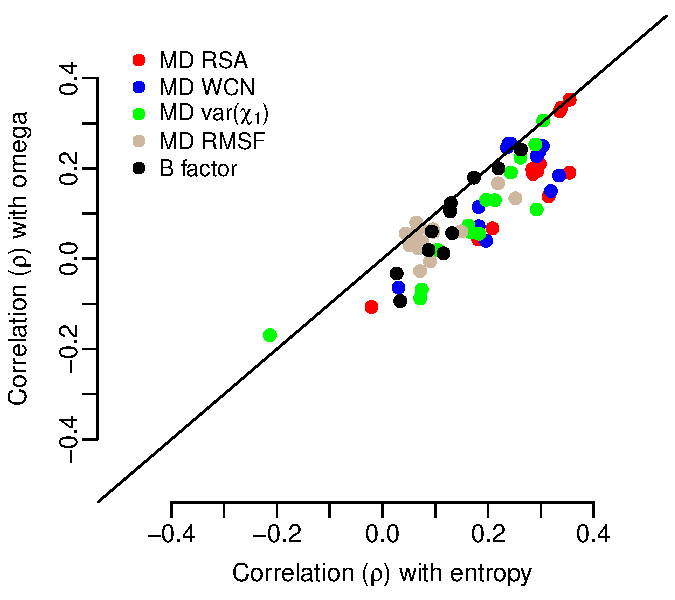
\includegraphics[width=4in]{cor_entropy_omega.pdf}
\end{center}
\caption{Spearman correlations of structural quantities with sequence entropy and with the evolutionary rate ratio $\omega$. All structural quantities generally predict as much as or more variation in sequence entropy than in $\omega$.}
\label{fig:cor_entropy_omega}
\end{figure}

\begin{figure}[tbh]
\begin{center}
       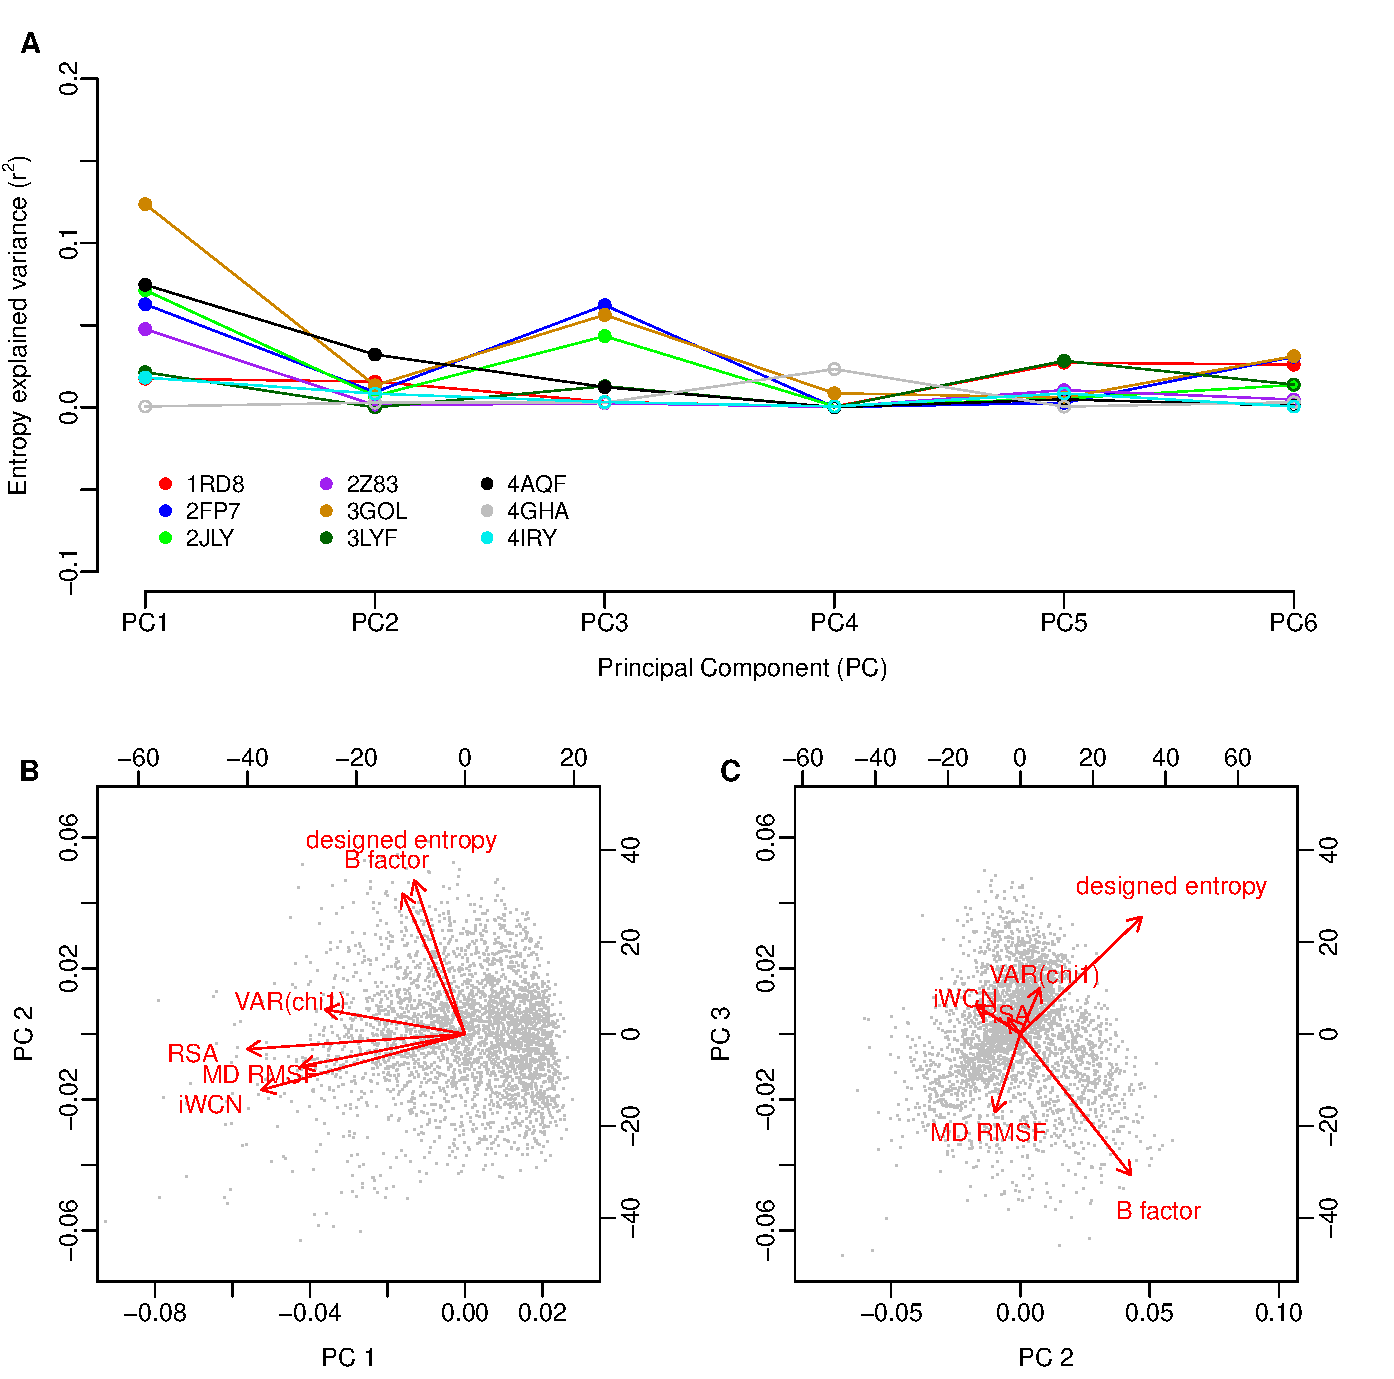
\includegraphics[width=6.5in]{PC_screen_entropy.pdf}
\end{center}
\caption{Principal Component (PC) Regression of sequence entropy against the structural variables. {\bf (A)} Variance in entropy explained by each principal component. For most proteins, PC1 and PC3 show the strongest correlations with sequence entropy. Significant correlations ($P<0.05$) are shown as filled symbols, and insignificant correlations ($P\leq0.05$) are shown as open symbols. {\bf (B)} and {\bf (C)} Composition of the three leading components. Red arrows represent the loadings of each of the structural variables on the principal components; black dots represent the amino acid sites in the PC coordinate system. The variables RSA, iWCN, MD RMSF, and Var($\chi_1$) load strongly on PC1 and weakly on PC2, while B factor and designed entropy load strongly on PC2 and weakly on PC1. Interestingly, B factor and designed entropy also load strongly on PC3, but in opposite directions.}
\label{fig:cor_entropy_PC_screen}
\end{figure}


\clearpage

\newpage
\section*{Supplementary Figures}

\centerline{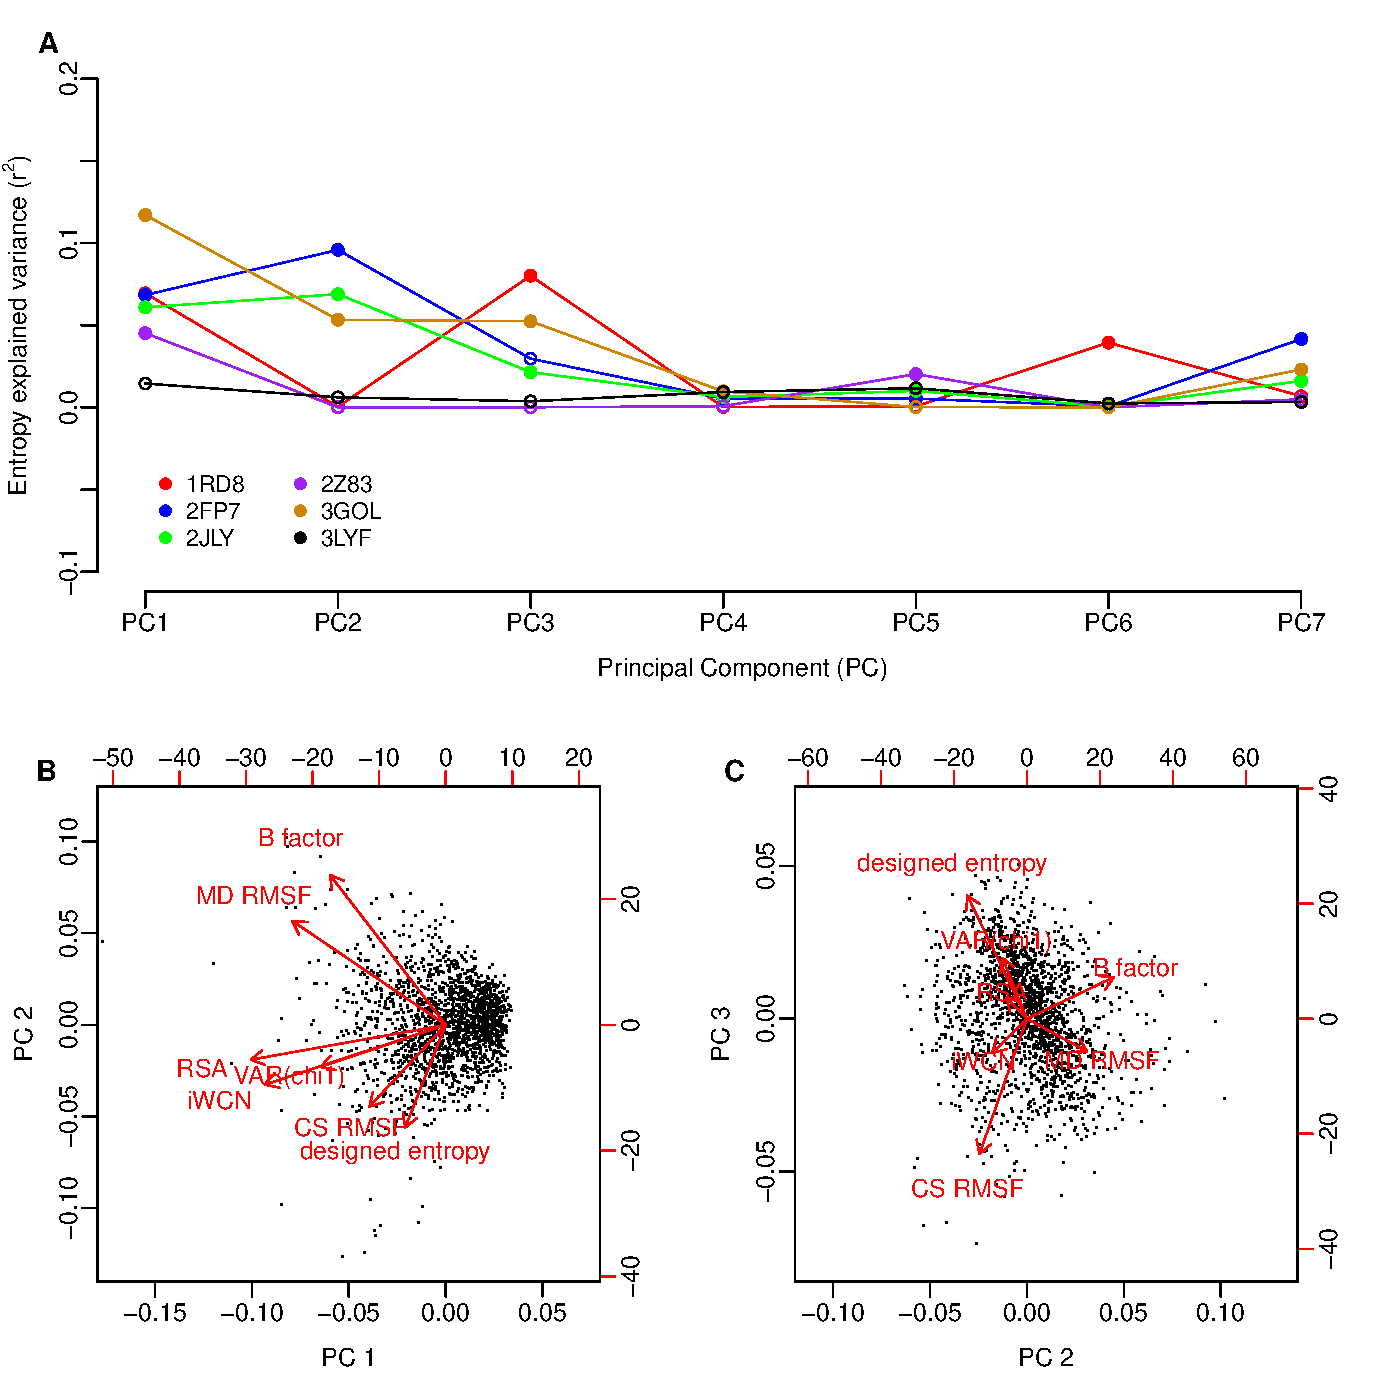
\includegraphics[width=6.5in]{PC_screen_entropy_CSrmsf.pdf}}
\noindent \textbf{Fig. S1} Principal Component (PC) Regression of sequence entropy against the structural variables, including CS RMSF. {\bf (A)} Variance in entropy explained by each principal component. For most proteins, PC1 and either PC2 or PC3 show the strongest correlations with sequence entropy. Significant correlations ($P<0.05$) are shown as filled symbols, and insignificant correlations ($P\leq0.05$) are shown as open symbols. {\bf (B)} and {\bf (C)} Composition of the three leading components. Red arrows represent the loadings of each of the structural variables on the principal components; black dots represent the amino acid sites in the PC coordinate system.
\customlabel{fig:cor_entropy_PC_screen_CSrmsf}{S1}


\newpage
\centerline{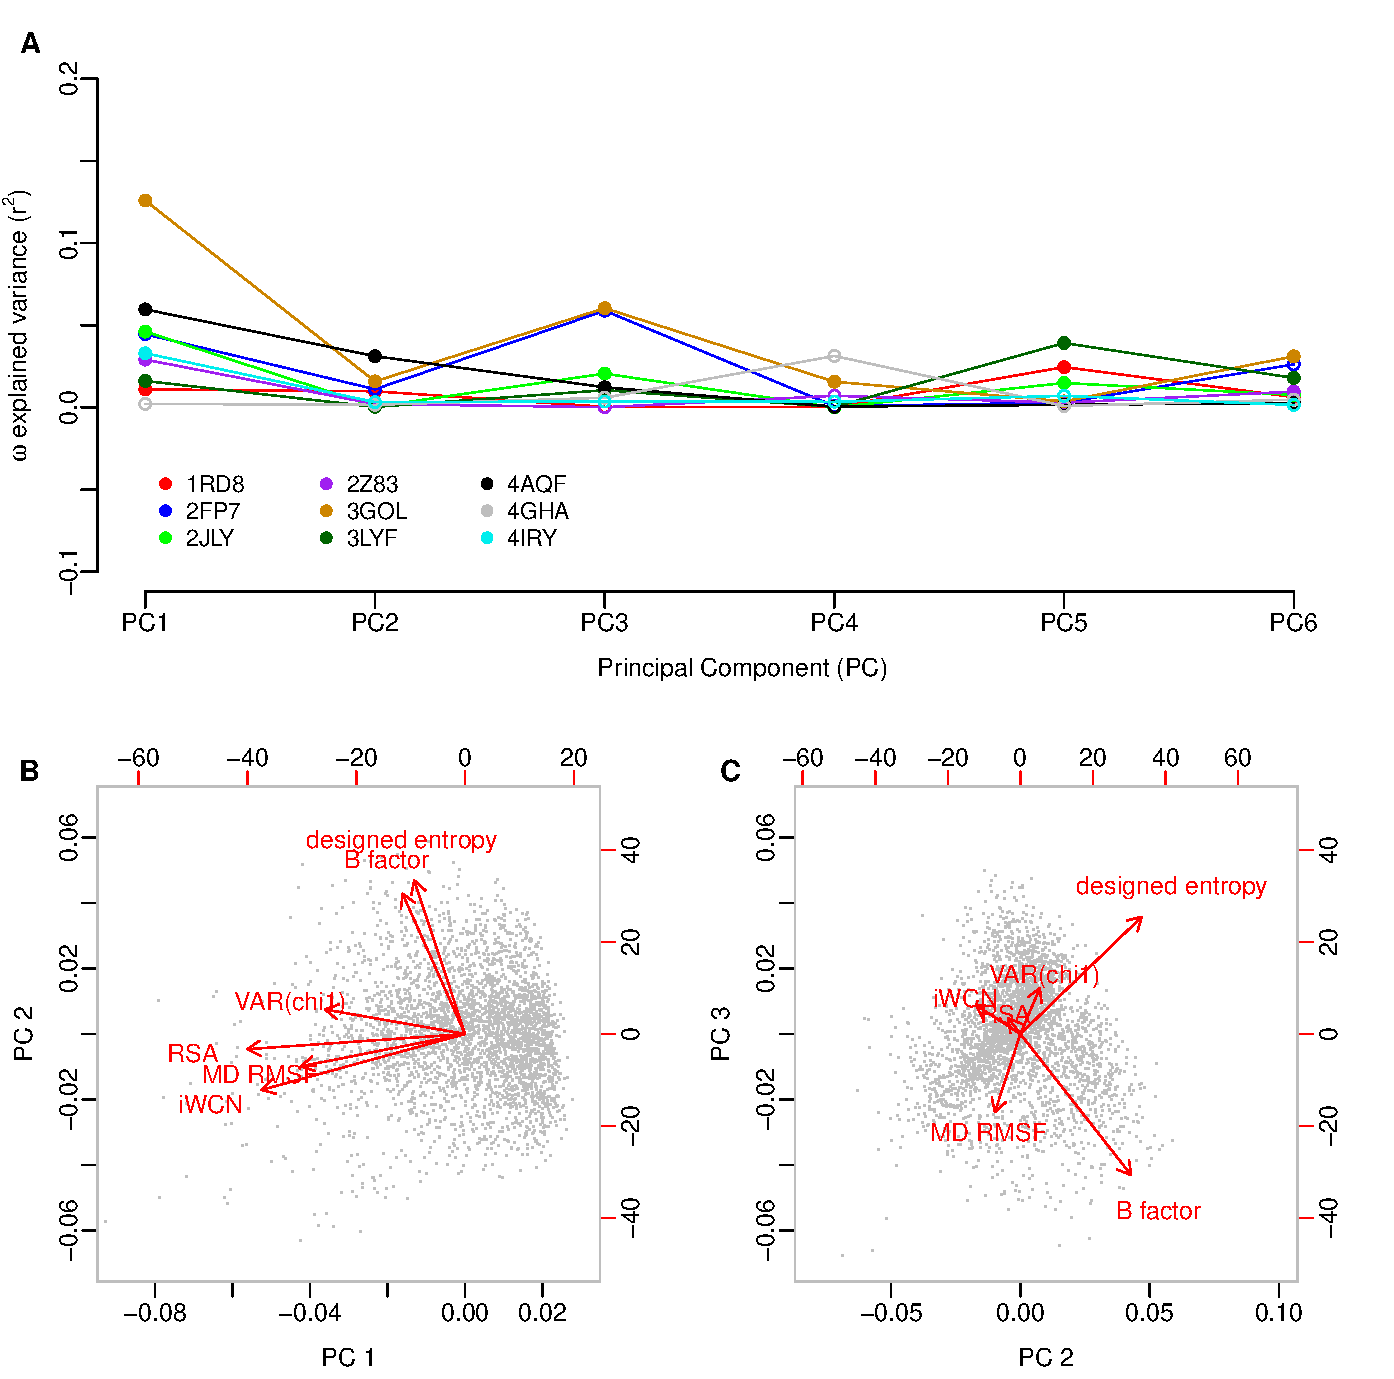
\includegraphics[width=6.5in]{PC_screen_omega.pdf}}
\noindent \textbf{Fig. S2} Principal Component (PC) Regression of $\omega$ against the structural variables. {\bf (A)} Variance in $\omega$ explained by each principal component. For most proteins, PC1 and PC3 show the strongest correlations with $\omega$. Significant correlations ($P<0.05$) are shown as filled symbols, and insignificant correlations ($P\leq0.05$) are shown as open symbols. {\bf (B)} and {\bf (C)} Composition of the three leading components. Red arrows represent the loadings of each of the structural variables on the principal components; black dots represent the amino acid sites in the PC coordinate system. Note that parts B and C are identical to those shown in Figure~\ref{fig:cor_entropy_PC_screen}.
\customlabel{fig:cor_omega_PC_screen}{S2}


\newpage
\centerline{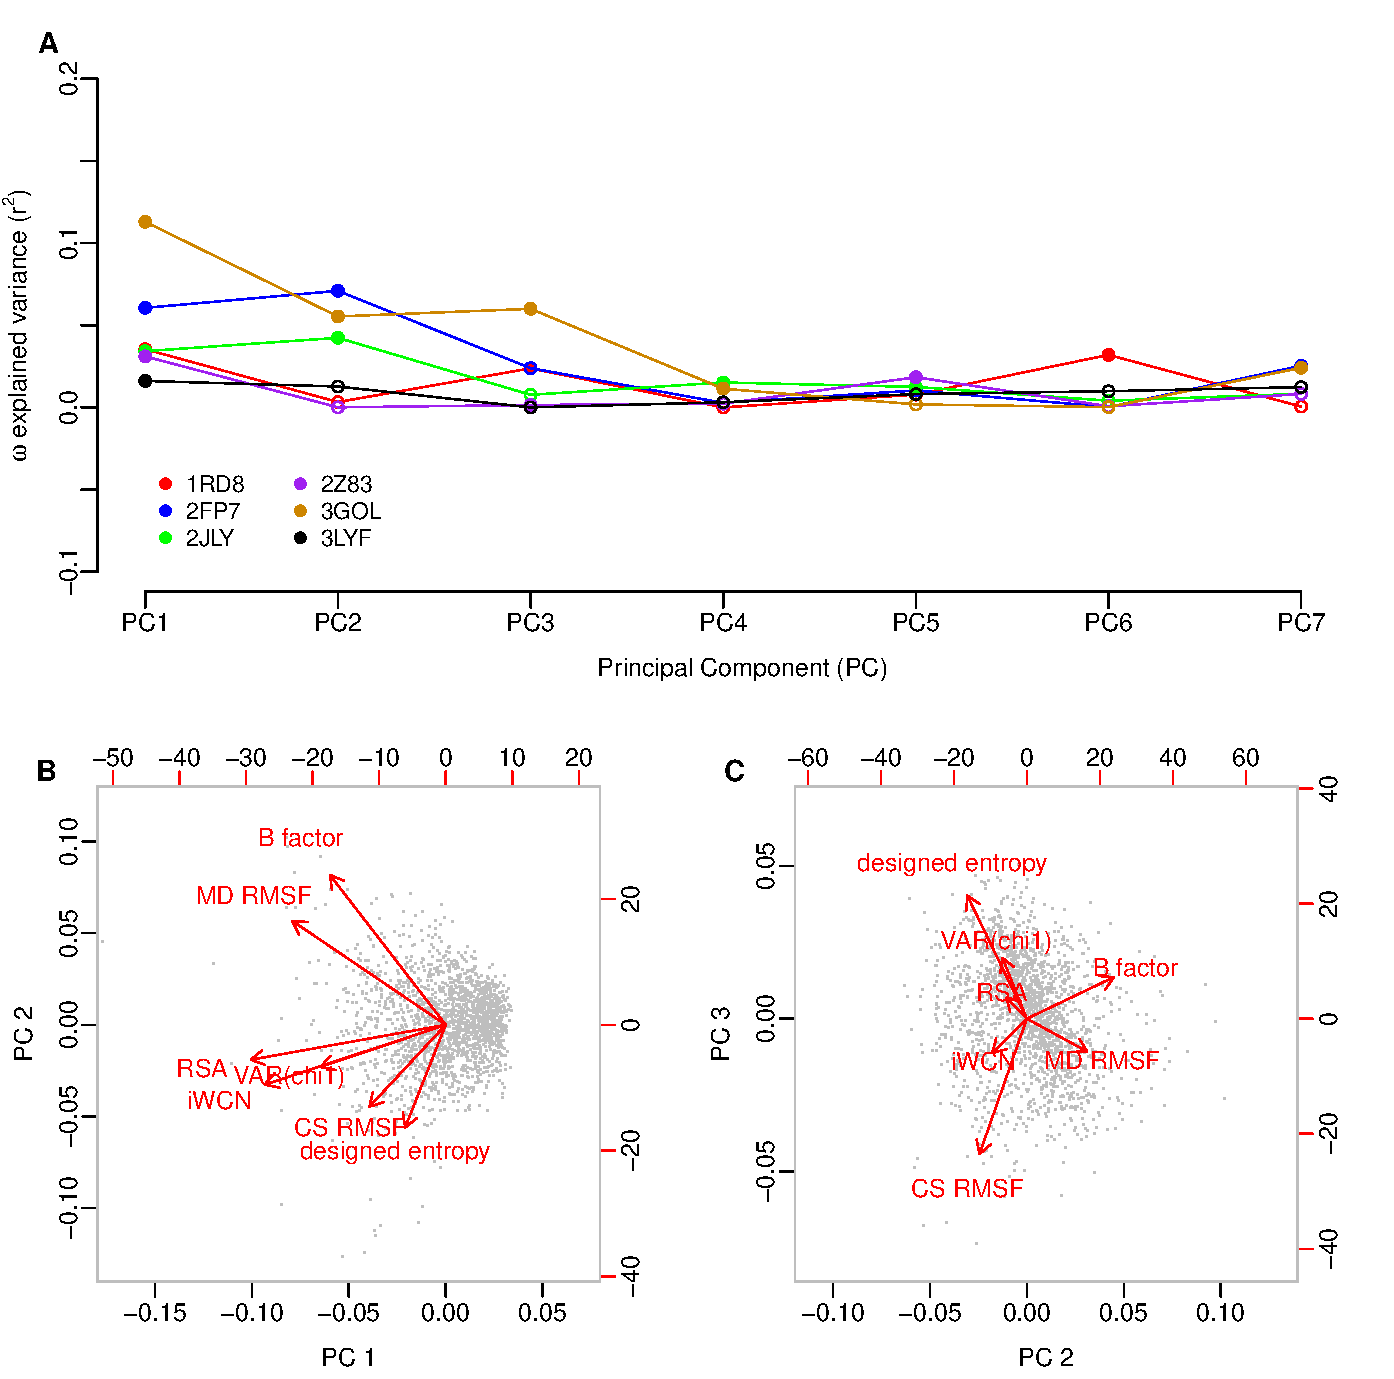
\includegraphics[width=6.5in]{PC_screen_omega_CSrmsf.pdf}}
\noindent \textbf{Fig. S3} Principal Component (PC) Regression of $\omega$ against the structural variables, including CS RMSF. {\bf (A)} Variance in $\omega$ explained by each principal component. For most proteins, PC1 and either PC2 or PC3 show the strongest correlations with $\omega$. Significant correlations ($P<0.05$) are shown as filled symbols, and insignificant correlations ($P\leq0.05$) are shown as open symbols. {\bf (B)} and {\bf (C)} Composition of the three leading components. Red arrows represent the loadings of each of the structural variables on the principal components; black dots represent the amino acid sites in the PC coordinate system. Note that parts B and C are identical to those shown in Figure~\ref{fig:cor_entropy_PC_screen_CSrmsf}.
\customlabel{fig:cor_omega_PC_screen_CSrmsf}{S3}


\end{document}
